
\section{Monday for MAT3006}\index{Monday_lecture}

\subsection{Applications on the Tonell's and Fubini's Theorem}
\begin{theorem}[Tonell]
Let $f:\mathbb{R}^2\to[0,\infty]$ be a measurable function (i.e., $f^{-1}((a,\infty])\in\mathcal{M}\otimes\mathcal{M}$), then
\[
\int f\diff\pi= \int \left(\int f(x,y)\diff x\right)\diff y
=
\int\left(\int f(x,y)\diff y\right)\diff x
\]
\end{theorem}

\begin{theorem}[Fubini]
Let $f:\mathbb{R}^2\to[-\infty,\infty]$ be integrable (i.e., $f=f^+-f^-$ with $f^{\pm}:\mathbb{R}^2\to[0,\infty]$ measurable and $\int f^{\pm}\diff x<\infty$), then
\[
\int f\diff \pi = \int \left(\int f(x,y)\diff x\right)\diff y
=
\int\left(\int f(x,y)\diff y\right)\diff x
\]
\end{theorem}

\begin{corollary}\label{cor:15:2}
Suppose that $f:\mathbb{R}^2\to[-\infty,\infty]$ is measurable, and either 
\begin{subequations}
\begin{equation}\label{Eq:15:1:a}
\int\left(\int |f(x,y)|\diff x\right)\diff y
\end{equation}
or
\begin{equation}\label{Eq:15:1:b}
\int\left(\int |f(x,y)|\diff y\right)\diff x
\end{equation}
\end{subequations}
 exists, then $f$ is integrable, and the result of Fubini follows.
(i.e., one can switch the order of integration as long as the integral of $|f|$ exists)
\end{corollary}
\begin{proof}
If (\ref{Eq:15:1:a}) or (\ref{Eq:15:1:b}) exists~(is finite), then Tonell's Theorem implies that $|f|$ is integrable, which implies $f$ is integrable.

Therefore, the assumption of Fubini's theorem holds, and the proof is comptete.
\end{proof}
\begin{remark}
The advantage for corollary~(\ref{cor:15:2}) is that computing (\ref{Eq:15:1:a}) or (\ref{Eq:15:1:b}) is easier than showing the integrability of $f$ in general. 
\end{remark}

\begin{example}
Compute the double integral
\[
\int_0^1\int_0^x\sqrt{\frac{1-y}{x-y}}\diff y\diff x.
\]
Construct the function $f(x,y):=\sqrt{\frac{1-y}{x-y}}\mathcal{X}_E(x,y)$, with $E$ shown in  Fig.~(\ref{fig:15:1}).
\begin{figure}[H]
\centering
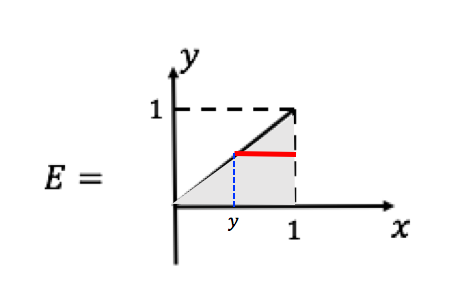
\includegraphics[width=0.4\textwidth]{week15/f_40}
\caption{Illustration for integral domain $E$}
\label{fig:15:1}
\end{figure}
We want to compute $\int f(x,y)\diff\pi$ and show that
\[
\int_0^1\int_0^x\sqrt{\frac{1-y}{x-y}}\diff y\diff x = \int f(x,y)\diff\pi.
\]
\begin{itemize}
\item
Consider the integral
\begin{subequations}
\begin{align}
\int\left(\int f(x,y)\diff x\right)\diff y &=\int_0^1\left(
\int_y^1\sqrt{\frac{1-y}{x-y}}\diff x
\right)\diff y\label{Eq:15:3:a}\\&=\int_0^1\sqrt{1-y}\left(\int_y^1\frac{1}{\sqrt{x-y}}\diff x\right)\diff y\\
&=\int_0^1\sqrt{1-y}\left(
\int_0^{1-y}\frac{1}{\sqrt{t}}\diff t
\right)\diff y\\
&=\int_0^1\sqrt{1-y}\cdot(2\sqrt{1-y})\diff y\\
&=2\int_0^1(1-y)\diff y\\
&=1
\end{align}
where the justification of (\ref{Eq:15:3:a}) is from Fig.~(\ref{fig:15:1}).
\end{subequations}
\item
Therefore, $\int(\int|f(x,y)|\diff x)\diff y<\infty$. Mreover, $f$ is continous on $E^\circ$, i.e., measurable on $E^\circ$~(it's clear that a continous function is measurable). Since $\partial E$ is null, we imply $f$ is measurable on $E:=E^\circ\cup\partial E$.
\item
Therefore, the assumption of Corollary~(\ref{cor:15:2}) holds, and we imply that
\[
\int\left(\int f(x,y)\diff y\right)\diff x = \int\left(\int f(x,y)\diff x\right)\diff y
\]
It's clear that 
\[
\int_0^1\int_0^x\sqrt{\frac{1-y}{x-y}}\diff y\diff x = \int\left(\int f(x,y)\diff y\right)\diff x,
\]
and therefore
\[
\int_0^1\int_0^x\sqrt{\frac{1-y}{x-y}}\diff y\diff x = 1.
\]
\end{itemize}
\end{example}
\paragraph{Process of Completion}
We have two measures on $\mathbb{R}^2$:
\begin{itemize}
\item
$\mathcal{M}\otimes\mathcal{M}$, and
\item
$\mathcal{M}_{\mathbb{R}^2}$, given by
\[
\mathcal{M}_{\mathbb{R}^2} = 
\{E\subseteq\mathbb{R}^2\mid m^*(A)=m^*(A\cap E)+m^*(A\cap E^c)\text{ for all subsets $A\subseteq\mathbb{R}^2$}\}
\]
\end{itemize}
Here $\mathcal{M}_{\mathbb{R}^2}$ equals the completion of $\mathcal{M}\otimes\mathcal{M}$, i.e.,
all $E\subseteq\mathcal{M}_{\mathbb{R}^2}$ can be decomposed as
\[
E = B\cup(E\setminus B),
\]
where $B\in\mathcal{M}\otimes\mathcal{M}$ and $E\setminus B\in \mathcal{M}_{\mathbb{R}^2}$ with $\pi(E\setminus B)=0$.

Question: does Tonell's theorem holds for (Lebesgue) measurable functions $f:\mathbb{R}^2\to[0,\infty]$ (i.e., $f^{-1}((a,\infty])\in \mathcal{M}_{\mathbb{R}^2}$ for any $a\in[0,\infty)$?)

Answer: Yes.
To see so, we just need the following proposition
\begin{proposition}
Let $(\mathbb{R}^2,\mathcal{M}_{\mathbb{R}^2},\pi)$ be the Lebesgue measure on $\mathbb{R}^2$, and $N\in\mathcal{M}_{\mathbb{R}^2}$ be such that $\pi(N)=0$.
Then for almost all values of $x\in\mathbb{R}$, $N_x\in\mathcal{M}$ and $m_Y(N_x)=0$.
\end{proposition}
\begin{proof}
For $N\in\mathcal{M}_{\mathbb{R}^2}$. By hw3, there exists $B'\in\mathcal{M}\otimes\mathcal{M}$ such that $N\subseteq B'$, with
\[
\pi(B')=\pi(N).
\]
If $N$ is null, then $\pi(B')=0$. By Tonell's theorem on $M\otimes\mathcal{M}$, we imply
\[
\pi(B') =\int m_Y(B_x')\diff x = \int m_X(B_y')\diff y=0
\]
Therefore, $m_Y(B_x')=0$ for almost all $x\in\mathbb{R}$.
Since $N\subseteq B'$, we imply $N_x\subseteq B_x'$, i.e., $N_x$ is also a null set.
Therefore, $N_x\in\mathcal{M}$ and $m_Y(N_x)=0$.
\end{proof}

\begin{example}
Consider the integral
\[
\int_0^\infty\int_0^\infty ye^{-y^2(1+x^2)}\diff y\diff x
\]
Define $f(x,y)=  ye^{-y^2(1+x^2)}$, which is continous on $(0,\infty)\times(0,\infty)$, and therefore measurable.
It follows that 
\begin{subequations}
\begin{align}
\int_0^\infty\int_0^\infty f(x,y)\diff y\diff x
&=\int_0^\infty\left(
\lim_{n\to\infty}\int_0^nf(x,y)\diff y
\right)\diff x\label{Eq:15:3:a}\\
&=\int_0^\infty\left(
\frac{1}{1+x^2}\frac{1}{2}
\right)\diff x\label{Eq:15:3:b}\\
&=\lim_{n\to\infty}\int_0^n\frac{1}{2}\frac{1}{1+x^2}\diff x\label{Eq:15:3:c}\\
&=\frac{\pi}{4}\label{Eq:15:3:d}
\end{align}
where (\ref{Eq:15:3:a}) is by applying MCT I on the function $f(x,y)\mathcal{X}_{[0,n]}$;
(\ref{Eq:15:3:b}) and (\ref{Eq:15:3:d}) is by computation;
(\ref{Eq:15:3:c}) is by applying MCT I on the function $\frac{1}{1+x^2}\frac{1}{2}\mathcal{X}_{[0,n]}$.
\end{subequations}

By corollary~(\ref{cor:15:2}), 
\[
\int_0^\infty\int_0^\infty ye^{-y^2(1+x^2)}\diff x\diff y=\frac{\pi}{4}
\]
Or equivalently,
\[
\int_0^\infty ye^{-y^2}\int_0^\infty e^{-x^2y^2}\diff x\diff y=\frac{\pi}{4}
\]
By applying MCT I on $e^{-x^2y^2}\mathcal{X}_{[0,n]}$, we have
\[
\int_0^\infty ye^{-y^2}\lim_{n\to\infty}\int_0^n e^{-x^2y^2}\diff x\diff y=\frac{\pi}{4}
\]
By change of variable with $t = xy$, we imply
\[
\int_0^\infty ye^{-y^2}\lim_{n\to\infty}\frac{1}{y}\int_0^{ny} e^{-t^2}\diff t\diff y=\frac{\pi}{4}
\]
Or equivalently,
\[
\int_0^\infty e^{-y^2}\int_0^\infty e^{-t^2}\diff t\diff y=\frac{\pi}{4}
\]
Therefore, we conclude that
\[
\left(\int_0^\infty e^{-y^2}\diff y\right)^2 = \frac{\pi}{4}\implies
\int_0^\infty e^{-x^2}\diff x = \frac{\sqrt{\pi}}{2}
\]
\end{example}


\subsection{Final Review}
Test: Tuesday, 9:00 - 11:30 am

Venue: TD105

Except ODE, i.e., Picard-Lindorf Theorem.

Contraction theorem and Weierstrass theorem will be tested.

Lucky: choose three oringinal problems from tutorial (question: in BB?)

Theorem mentioned today, how to use, and remember how to proof.

Some problems, Fotou;s lemma, MCT, DCT, Stone-weierstrasss theorem.

How say? how to proof?

8 problems at most.

\begin{enumerate}
\item
Part I: metric space, and set theorem.
\begin{itemize}
\item
a metric $d:X^2\to\mathbb{R}^+\cup\{0\}$.
Properties:
\begin{itemize}
\item
Non-negativity, i.e., $d\ge0$, and $d(x,y)=0$ iff $x=y$.
\item
Symmetry: $d(x,y)=d(y,x)$
\item
Triangle inequality: $d(x,y)\le d(x,z)+d(z,y)$ 
\end{itemize}
\item
An open set $G\subseteq X$: for all $x\in G$, there exists $\rho>0$, such that $B_{\rho}(x)=\{y\in X\mid d(y,x)<\rho\}\subseteq G$.

An interior point $x_0\in G$: for some $\varepsilon>0$, $B_{\varepsilon}(x_0)\subseteq G$.

Important: If all the $x$ in $G$ are interior points, then $G$ is open
\item
A closed set $G^c$, when $G$ is open
\item
A limit point $x_0\in G^c$: for all $\varepsilon>0$, there exists $y\in X$ and $y\ne x_0$ such that
\[
y\in B_{\varepsilon}(x_0)
\]
Important: If all the points in $G^c$ are limit points, then $G^c$ is closed.
\item
A compact set $K\subseteq X$:
every open cover of $K$ has a finite subcover.

In Euclidean space $(\mathbb{R}^n)$, when $K$ is closed and bounded

Important: In metric space $(X,d)$, every sequence $\{x_n\}$ in $K$ has a subsequence $\{x_{n_i}\}\to x\in K$ as $i\to\infty$
\item
A complete space $X$:
all the Cauchy sequence converges in $X$.

Counter-example for in-complete space
\item
Compactness implies completeness, and further completeness implies closedness
\item
Important: Stone-Weierstrass Theorem: 
what is Stone-Weierstrass approximation Theorem.
Not full version, but approximation theorem.

A sub-algebra: $\mathcal{A}\subseteq\mathcal{C}(X)$.

$\mathcal{A}$ is dense in $\mathcal{C}(X)$ ($X$ is compact), i.e., $\bar{\mathcal{A}}=\mathcal{C}(X)$.

Equivalent to say $\mathcal{A}$ is equipped with two properties:
\begin{itemize}
\item
separation property
\item
non-vanishing property
\end{itemize}
Weierstrass Approximation Theorem, read the proof for polynomials
\item
Arzela-Ascoli Theorem: 
for a closed subset $\mathcal{F}\subseteq\mathcal{C}(K)$, where $K$ is compact in $\mathbb{R}^n$, then 
$\mathcal{F}$ is compact, i.e., $\mathcal{F}$ is bounded and equi-continuous.

Equi-continuity: for all $\varepsilon>0$, there exists $\delta>0$ such that 
\[
|f(x)-f(y)|<\varepsilon,\quad
\text{provided that }|x-y|<\delta, f\in\mathcal{F}
\]
how to find $\delta$.
\item
Baire-Category Theorem:
A subset sequence $\{E_n\}$ of complete $(X,d)$ is nowhere dense implies that $\cup_nE_n$ has empty interior.

\end{itemize}
\item
Measure Theory:
\begin{itemize}
\item
Outer measure: $m^*(\cdot)$, other kind of measure, definition
\[
m^*(E) = \inf\left\{
\sum_nm(I_n)\middle|
E\subseteq\bigcup_{n=1}^{\infty}I_n\text{ open rectangles}
\right\}
\]
For Euclidean space, $m(I_n) = \prod_{i=1}^n(b_i^{(n)} - a_i^{(n)})$ and $I_n = $.
\item
Inner measure:
\[
m_*(E) = \sup\left\{
\sum_nm(I_n)
\middle|
\sqcup_{n=1}^\infty I_n\subseteq E,
\quad
\text{$I_n$'s are disjoint union}
\right\}
\]
relate to Riemann integral
\item
Lebesgue measurable: Carthedory extension theorem
\[
m^*(S) = m^*(S\cap E) + m^*(S\cap E^c)\implies m^*(E) = m(E)
\]
(Important) Equivalent proposition:
For any $A\subseteq E$ and $B\in E^c$, 
\[
m^*(A\cup B) = m^*(A)+m^*(B)
\]

Examples of non-measurable: Vitali Set
\item
Measurable Function: $f:X\to Y$,
\[
f^{-1}(E)=\{x\in X\mid f(x)\in E\}\in\mathcal{F},\forall E\in\mathcal{G},
\]
where $\mathcal{F}$ and $\mathcal{G}$ are $\sigma$-algebras w.r.t $X,Y$.

Lebesgue Measurable~(easier):
$f:X\to\mathbb{R}$.
\[
\{x\in X:f(x)>a\}\text{ is measurable for }\forall a\in\mathbb{R}
\]
Equivalent to $\{x\in X\mid f(x)\le a\}$.
\item
Important: almost everywhere convergence:
$f_n\to f$ a.e., i.e., $m\{x\in X:\lim_{n\to\infty}f_n(x)\ne f(x)\}=0$.

Convergent in measure: 
$f_n\to f$ is equivalent to say
\[
\lim_{n\to\infty}m\{x\in X\mid |f_n(x)-f(x)|<\varepsilon\}=0,\quad\forall\varepsilon>0
\]
\item
Part III: Lebesgue Integral.

Simple function: $\phi:X\to\mathbb{R}$ by 
\[
\phi(x) = \sum_{i=1}^n\alpha_i\mathcal{X}_{A_i}(x)
\]
where $a_1,\dots,a_n\in\mathbb{R}$ and $A_1,\dots,A_n\subseteq X$ are disjoint, with
\[
\mathcal{X}_{A_i}(x)=
\]
$\int_{X}\mathcal{X}_{A_i}\diff m = m(A_i)$
\item
Lebesgue integral for $\phi$ on $E\subseteq X$:
\[
\int_E\phi\diff m =\sum_{i=1}^na_im(A_i\cap E)
\]
\item
Lebesgue integral for non-negative $f$:
\[
\int_Ef\diff m =  \sup\{\int_E\phi\diff m \mid 0\le\phi\le f\}
\]
\item
For general $f$, $f = f^+- f^-$, with
\[
f^+=\left\{
\begin{aligned}
f,&\quad f>0\\
0,&\quad\text{otherwise}
\end{aligned}
\right.
\]
\item
If $\int|f|\diff m<\infty$, then $f$ is Lebesgue integrable.
\end{itemize}
\item
\begin{itemize}
\item
No proof for Fatuou's lemma.

For non-negative $\{f_n\}$ on measurable $X,$
\[
\int_X\lim_{n\to\infty}\int f_n\diff m \le \lim_{n\to\infty}\int \int_Xf_n\diff m
\]
\item
Proof is important: Monotonce convergence theorem:
Assumption:
\begin{itemize}
\item
$f_n:X\to[0,\infty]$
\item
$f_n\le f_{n+1}$
\item
$f_n\to f$ a.e.
\end{itemize}
Conclusion:
\[
\lim_{n\to\infty}\int_Xf_n\diff m =\int_X\lim_{n\to\infty}f_n\diff m = \int _Xf\diff m
\]
\item
Dominated Convergence Theorem:
\begin{itemize}
\item
$|f_n|\le g$, where $g$ is Lebesgue measurable
\item
$f_n\to f$ a.e.
\end{itemize}
\item
Fubini's Theorem: 
$(X,Y)$ is measurable, $(X\times Y)$, $f$ is measurable function.
If 
\[
\int_{X\times Y}|f|\diff(x,y) = \int _X\int_Y|f|\diff y\diff x = \int_Y\int_X|f|\diff x\diff y
\]
then
\[
\int_{X\times Y}f\diff(x,y) = \int _X\int_Yf\diff y\diff x = \int_Y\int_Xf\diff x\diff y
\]
how does this theorem expresses in Riemann integral.

Proof in Riemann integral case.

Check counter-examples.
\end{itemize}

\end{enumerate}





















